%===============================================================================
% $Id: ifacconf.tex 19 2011-10-27 09:32:13Z jpuente $
% Template for IFAC meeting papers
% Copyright (c) 2007-2008 International Federation of Automatic Control
%===============================================================================
\documentclass{ifacconf}

\usepackage{graphicx}      % include this line if your document contains figures
\usepackage{natbib}        % required for bibliography
\usepackage{subfigure}
\usepackage{enumerate}
%===============================================================================
\begin{document}
\begin{frontmatter}

\title{THE EMBEDDED ELECTRONICS SYSTEM OF DORIS: A MOBILE ROBOT FOR INSPECTION AND MONITORING OF
OFFSHORE FACILITIES\thanksref{footnoteinfo}}
% Title, preferably not more than 10 words.

\thanks[footnoteinfo]{This work is supported primarily by Petrobras S.A. and
Statoil Brazil Oil \& Gas Ltda under contract COPPETEC 0050.0079406.12.9
(ANP-Brazil R \& D Program), and in part by the Brazilian research agencies CNPq
and FAPERJ}

\author[1]{Ramon R. Costa}
\author[1]{Renan S. Freitas}
\author[1]{Marco F. S. Xaud}
\author[1]{Ighor Marcovistz}
\author[1]{Alex F. Neves}
\author[1]{Rafael O. Farias}
\author[1]{Guilherme P. S. Carvalho}
\author[1]{Liu Hsu}
\author[1]{Eduardo V. L. Nunes}
\author[1]{Alessandro J. Peixoto}
\author[1]{Fernando Lizarralde}
\author[4]{P{\aa}l From}
\author[1]{Gustavo Freitas}
\author[1]{Eduardo A. B. da Silva}
\author[1]{Sergio L. Neto}
\author[2]{Maur{\'i}cio Galassi}
\author[3]{Anders R{\o}yr{\o}y}


% Op��o 1 de filia��o sem email
%  \address[1]{Electrical
% Engineering Department, COPPE UFRJ, Rio de Janeiro, Brazil }
% \address[2]{Research and Development Center, Petrobras/CENPES,
% Rio de Janeiro, Brazil }
% \address[3]{TPD RD New Development Solutions, Statoil ASA, Bergen, Norway }
%\address[4]{Mathematical Sciences and Technology Department, Norwegian
%University of Life Sciences, Oslo, Norway }

%% Op��o 2 de filia��o com email
  \address[1]{Electrical
 Engineering Department, COPPE UFRJ, Rio de Janeiro, Brazil (renan028@poli.ufrj.br, marco.fernandes@poli.ufrj.br, imtz@poli.ufrj.br, alexfneves@poli.ufrj.br, rafael.o.faria@gmail.com, guilherme\_carvalho@poli.ufrj.br,\{liu,eduardo,jacoud,fernando,gfreitas,ramon\}@coep.ufrj.br, \{eduardo,sergioln\}@smt.ufrj.br)}
 \address[2]{Research and Development Center, Petrobras/CENPES,
 Rio de Janeiro, Brazil (mauricio.galassi@petrobras.com.br)}
 \address[3]{TPD RD New Development Solutions, Statoil ASA, Bergen, Norway (aroy@statoil.com)}
\address[4]{Mathematical Sciences and Technology Department, Norwegian
University of Life Sciences, Oslo, Norway (pafr@umb.no)}

\begin{abstract}                % Abstract of not more than 250 words.
DORIS is a research project which endeavors to design and implement a mobile
robot for remote supervision, diagnosis, and data acquisition on offshore
facilities. The proposed system is composed of a rail-guided robot capable of
carrying different sensors through the inspected area. This paper presents a
general overview of the robot, and a description of the developed embedded
electronics, power supply system and software architecture. Initial results
with teleoperated navigation validate the concepts considered so far and
rise several challenges for future works.
\end{abstract}

\begin{keyword}
mobile robots; field robotics; embedded electronics; power supply; robotic
software architecture;
\end{keyword}

\end{frontmatter}
%===============================================================================

\section{Introduction}
The Oil \& Gas demand will grow rapidly in the next decades (\cite{wna}) and the
need to obtain the resources from hostile environments will increase operation
cost. In order to be competitive and to improve their profit, oil \& gas
companies are looking for new technologies to reduce the labor costs. The use
of robotics in inspection maintenance and repair operations in oil \& gas
facilities could greatly improve efficiency, health and safety, while
decreasing operational and logistics costs.

In the specific case of Brazil, the Oil \& Gas industry is growing at a high
pace. The recent discoveries of big oil fields in the pre-salt layer off the
Brazilian coast, located 300 km from the shore at depths of 5000 to 7000 km,
motivates the development of an offshore  production system with a high degree
of automation based on advanced robotics systems (\cite{presal}).

The work conditions on offshore
installations such as unfriendly atmosphere, unsheltered environment, heavy
wheather, extreme temperatures, constrained space, and the logistical issues
are serious financial obstacles for oil \& gas companies.
% It is highly expensive to have people working on the rig, as they
% must be housed and protected, there are costs with personal benefits such as
% health care, and the companies need to evacuate personnel quickly
% in case of an emergency.

Recent studies forecast a substantial decrease in the level of human operation
and an increase in automation on future offshore oil fields
(\cite{skourup2009robotized}). The studies also point out the potential increase
in efficiency and productivity with robot operators. Besides of the improvement in
Health, Safety, and Environment (HSE) conditions, as robots can replace humans
in tasks performed in unhealthy, hazardous, and confined areas (\cite{pal}).

\cite{chen} investigates the challenges of robotics and automation in oil
\& gas industry and lists the most important requirements for robotic systems
are:
\begin{itemize}
\item The atmospheric conditions on offshore platforms are quite unfriendly. The
hydrocarbon resources can generate explosive, toxic and corrosive gases. The
robot should be certified to operate in explosive environments.
\item Corrosive environments: splashy salty water, salty air and corrosive
chemicals.
\item Weather: wind with high speed, squalls, rain and hail. The
significant variations on ambient temperature and relative humidity are up to
100\%. Possibly highly radiant heat from process equipment and direct sunlight.
\item Constrained space and/or walkways. Complex structures such as pipes,
flanges, tanks, and stairways.
\end{itemize}

%There are different kinds of robots in the oil \& gas industry such as
%underwater pipeline repair robotic systems, robots for inspection of valve and
%lever position, gas level or leakage and acoustic anomalies monitoring, and
%robots for identify and locate fire.

Currently, the majority of robotic systems used in the Oil \& Gas industry are used for subsea tasks, such as mapping of the seabed, and inspection and repair of underwater equipment, risers and pipelines. However, recent research has focused on robotic applications on the topside of platforms to perform tasks such as inspection of valve and
lever position, gas level or leakage and acoustic anomalies monitoring, and
robots for identify and locate fire.

The MIMROex inspection robot (\cite{mimroex}) was developed and
tested by the Fraunhofer Institute of Manufacturing Engineering and Automation
(IPA). The robot is capable of safe navigation in offshore environments, and
autonomous execution of inspection tasks.

The Carnegie Mellon University inspection robot Sensabot (\cite{sensabot}) was
designed for severe weather and unfriendly atmosphere with corrosive, toxic and explosive
gases, being certified to operate in toxic, flammable and explosive environments. The robot includes the following sensors: (i) hydro carbon sensor; (ii)
pan/tilt/zoom camera for remote operations; (iii) temperature sensors; (iv)
vibration sensor for pumps, motors and bearings inspection; (v) microphone to
detect audible machinery problems; (vi) video camera to detect obstacles.

The SINTEF Topside Robotic System, developed in the robotic lab facility in
Trondheim, is an intelligent instrumentation system to enable onshore operators
to monitor and control all of the platform's processes
(\cite{kyrkjebo2009robotic}).

In this paper, we describe the DORIS project, which aims to develop a mobile
robot to perform monitoring and inspection in an
offshore platform. To this end, the system must be able to move throughout the
monitored environment carrying different sensors, analyzing sensor data
\emph{in loco} or storing it for a posterior analysis, and interpreting the
results. The sensors can identify abnormalities such as intruders in restricted
areas, abandoned objects, smoke, fire, and liquid and gas leakages.
Furthermore, the robot is able to make machinery diagnosis, read instruments,
and takes samples using an embedded
manipulator (\cite{cba}).

The paper is organized as follows: a general overview of the robot and its main
challenges are presented in Section \ref{sec:general_overview}, detailed
descriptions of the embedded electronics, the vehicle support system, power
supply system, and software architecture are taken in
Sections \ref{sec:electronics_overview},
\ref{sec:VSS}, \ref{sec:powersupply_overview}, and
\ref{sec:software} respectively.
In Section \ref{sec:results}, preliminary results are shown, and concluding
remarks are drawn in Section \ref{sec:conclusions}.

\section{General Overview}\label{sec:general_overview}

The DORIS robot is composed of a robot with cameras, microphones, gas,
vibration and temperature sensors, and a manipulator arm. The robotic device is
guided by a rail and both the robot and the rail follows a modularity concept.
Additional robot modules can be annexed to include other sensors, and the rail
track can be modified by adding or replacing rail segments, thus enabling
operation in different areas of the platform.

The robot will be controlled autonomously or by teleoperation. Task managing
can be either in automatic (programmed using a mission interface) or manual
mode (real-time remote operation). The teleoperation and monitoring
capabilities guarantee online access to the embedded sensors, providing
information about the surrounding environment and the robot operating
conditions with real-time processing. Figure~\ref{fig:DORIS-overview}
illustrates the operation in a production plant.


\begin{figure}[ht]
\centering
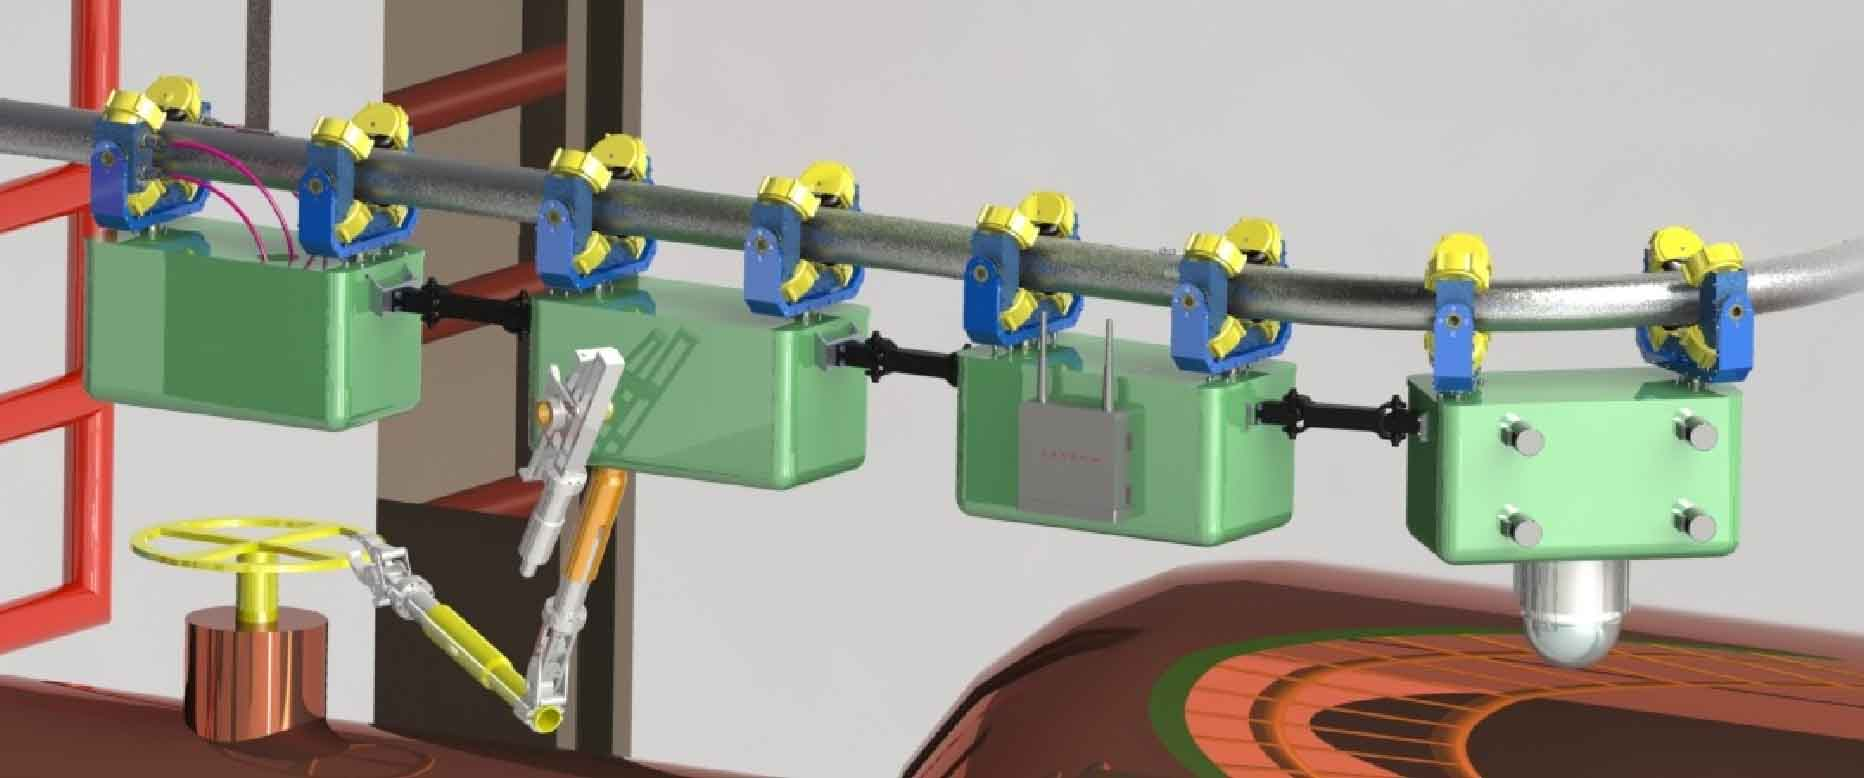
\includegraphics[width=8.4cm]{figs/zoom.jpg}
\caption{Illustration of the DORIS robot operating in a production plant}
\label{fig:DORIS-overview}
\end{figure}

The DORIS project can be divided into five subsystems: electronics, power
supply, software, mechanics and signal processing.

%-------------------------------------------------------------------------------------------------------------------------
%ELECTRONICS
%-------------------------------------------------------------------------------------------------------------------------
% The electronics subsystem is responsible for providing embedded computational
% support for the robot control, signal processing, task managing, and local and
% remote communication. The device motion is controlled through drivers that can
% receive position, velocity, or current setpoints. The embedded electronics has
% two printed circuit boards for the vehicle support system: energy distribution
% and monitoring, basic failure detection, emergency handling and devices'
% control.

%-------------------------------------------------------------------------------------------------------------------------
%POWER SUPPLY
%-------------------------------------------------------------------------------------------------------------------------
% The power supply system uses military-class lithium-ion batteries, which have
% small size and high energy capacity. In the first prototype of DORIS, four
% batteries are used to power the motors and two to power the other electronics
% components.


%-------------------------------------------------------------------------------------------------------------------------
%SOFTWARE
%-------------------------------------------------------------------------------------------------------------------------
% The main objective of the software subsystem is to allow the implementation of
% high- and low-level control of the robot. The tools used to develop DORIS
% software architecture must consider two important factors: they have to be
% commercially available, and provide modular functionalities. These requirements
% led to the adoption of Qt as the graphical interface framework ~\cite{qt},
% Robot Operating System (ROS) as the communication middleware ~\cite{ros}, and
% Ubuntu as the operating system.
%
% The software provides autonomous control (programmed tasks) and remote control
% through a Graphical User Interface (GUI) in the Host Control Base (HCB)
% computer. The HCB is composed of a set of processes running in parallel
% denominated ROS nodes, which can communicate with each other. To deal with this
% environment, a new software architecture called Robot Package Software is
% proposed, dividing the software into tools (graphical windows) and components
% (processing and communication unities), and grouping them into a dynamic
% library.

%-------------------------------------------------------------------------------------------------------------------------
%Mechanics
%-------------------------------------------------------------------------------------------------------------------------
The mechanics comprises the rail, the modules and the joints used to couple
them. Its design allows the robot to move smoothly in a 3D space and make a full
stop anywhere on the rail. Considering the severe corrosion and weather
conditions in offshore environments, the choice of materials is imperative for
the success of the project and certified solutions must be considered if available.

The robot is composed of two modules in its default configuration, but it is
conceived to be augmented with additional modules. The total weight
of this basic configuration is estimated at 50 kg. The speed of DORIS is expected to reach 1m/s.

The design incorporates the use of gimbals with wheels as guides for
the module on the rail. The use of two sets of gimbals provide mechanical compliance with rail curvatures, smoothness of the robot's base movement, and good weight distribution.

%-------------------------------------------------------------------------------------------------------------------------
%DSP
%-------------------------------------------------------------------------------------------------------------------------
The signal processing capabilities of the robot are: (a) Video: use
of multiple cameras (visible-light, infrared, panoramic and stereo) to detect
video anomalies such as abandoned objects, smoke, fire, liquid leakage, and
intruders. (b) Audio: detection of audio anomalies of impulsive nature, such as
an explosion, or the diagnosis of rotating machines based on energy and pitch
(fundamental frequency) signatures using a single or a array of microphones. (c)
Vibration analysis: use of acceleration sensors to diagnose the operation mode
of rotating machines, performing possible fault classification, such as
 misalignment and unbalancing operation. (d) Gas sensor: detection of gas
 leakages. (e) 3D mapping: environment 3D modeling using a laser sensor.

The main idea of all these signal processing features is to make the robot
perform an initial reference lap around the closed rail track, being manually
validated by a system operator. In the subsequent laps, all signal processing
algorithms compare the newly acquired signals with the reference data to detect
any form of anomaly, as indicated above. Once an anomalous behavior is
detected, an alarm is flagged to the system, which stores all associated data
for immediate or future diagnosis.

A more detailed presentation of the mechanical and signal processing systems can be found in \cite{OTC} and
\cite{cba}.

%-------------------------------------------------------------------------------------------------------------------------
%OTHER CHALLENGES
%-------------------------------------------------------------------------------------------------------------------------
Considering the robot functionalities and the aggressive offshore environment,
several challenges should be addressed. Temperatures in offshore facilities can
vary between $-30^{\circ}$C to $50^{\circ}$C, relative humidity can reach
100\%, and there may be splash water, salty air, storms, and high extensive
corrosion ~\cite{graf2007mobile}.

Concerning robustness and safety required to operate in classified areas, the
robot must be sealed against water and objects, resistant to a wide temperature
range, protected from impact and vibration, electrically shielded to avoid
explosion by ignition, and equipped with a monitoring system.

Another challenge is that the embedded computers must run heavy signal
processing algorithms, requiring high computational power. However, the power
supply subsystem must efficiently provide power and maintain a low level of
power consumption.

Further complications arise because the system is designed to move in confined
areas and have efficient wireless communication with operators, providing
online information of sensors data. Finally, the robot must have a modular and
flexible design, employing plug and play extensions.


\section{Embedded Electronics}\label{sec:electronics_overview}
The embedded electronics (EE) is composed of the following subsystems:
communication system, actuation system, sensor integration system, and vehicle
support system.

The \emph{communication system} is composed of: i) local Gigabit Ethernet
network for heavy data communication; ii) CAN (\emph{Controller Area Network})
for communication of control commands; iii) wireless technologies between the
robot and the remote control base located at the offshore facility. DORIS can
be remotely operated from this base via Wi-Fi IEEE 802.11n or via 2.4/5.0 GHz
radio links (upon Wi-Fi failures).

The Ethernet network has a star topology centralized by a OSI-Layer 2 Switch,
and connects DORIS main devices: i) computer; ii) three cameras (one with an
embedded microphone); iii) Wi-Fi access point (another one is needed at the
remote base); iv) \emph{Printed Circuit Boards} (PCBs). Together, Ethernet
network and Wi-Fi form a \emph{Local Area Network} (LAN) for real-time
communication and processing of heavy data amount, such as audio, video from all
cameras. In addition, this network topology allows easy expansion of the
Ethernet network for additional modules.

DORIS traction is taken by the \emph{actuation system}, which is composed of:
i) 4 motor packs, each containing a 200 W EC-4pole Maxon brushless
motor, an encoder and a high power planetary gearhead; ii) 4 controller drivers;
iii) respective cable/connector set.
The actuation system is commanded by the DORIS computer via CAN bus, which
provides reliability, transmission security and appropriate speed to this
application (\cite{can}). Since the traction system generates a significant
amount of conductive noise, a galvanic opto-isolator is used between the CAN and the
computer to minimize interference on the rest of the EE system.
% Gustavo: Falar do Watchdog do alex

The sensor integration system is composed of all DORIS sensors and the interface
between devices and the computer. The subsystem enables inclusion,
reconfiguration and replacement of peripheral devices. The sensor data
integration is carried out by a high performance Intel\textregistered
Core\texttrademark i7 computer embedded in a PCIe/104 form factor board.

An overall scheme of DORIS EE system is shown in
figure~\ref{fig:EE-Communications}.

\begin{figure}
\begin{center}
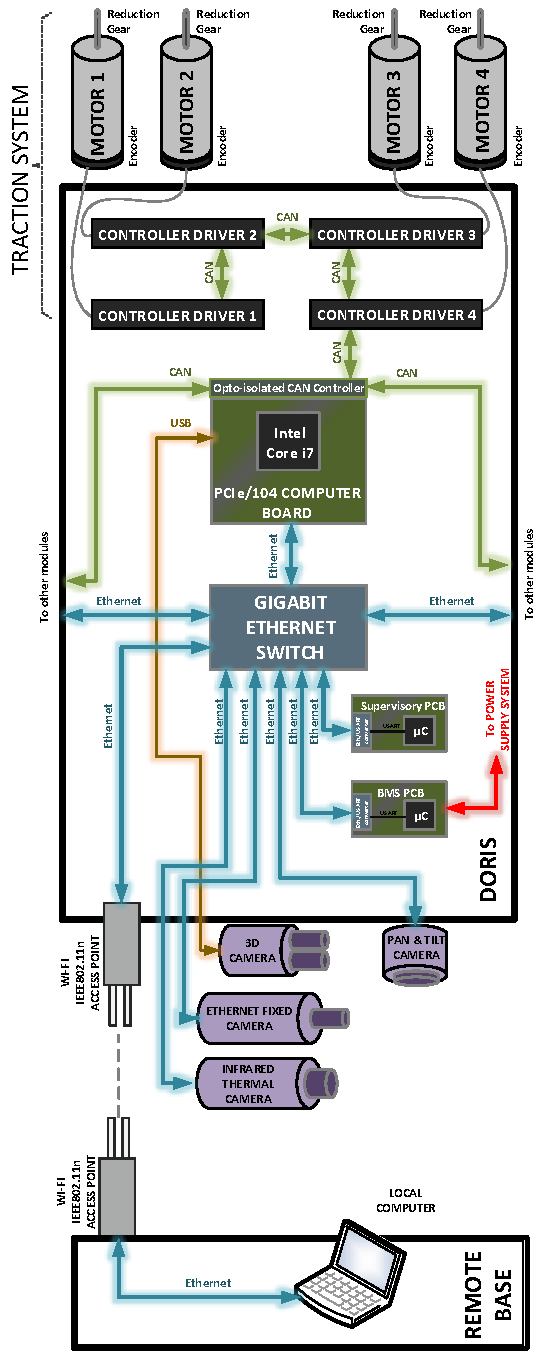
\includegraphics[width=8.4cm]{figs/EE-Communications.pdf}
\caption{DORIS embedded Electronics system: overall scheme}
\label{fig:EE-Communications}
\end{center}
\end{figure}

\subsection{Vehicle Support System}\label{sec:VSS}

The \emph{Vehicle Support System (VSS)} (\cite{MARIUS}) is composed of
microcontroller based PCBs for: failure detection; device protection;
energy distribution and monitoring; emergency handling. The VSS is designed for:

\begin{itemize}
    \item Failure detection is achieved by the monitoring of devices'
    current/voltage and module humidity/temp.
    \item Peripheral devices are protected against overcurrent by fuses and
    solid-state relays, which can be turned on/off at any time automatically,
    upon a detected failure, or manually via operator.
    \item Energy distribution and monitoring is achieved by the \emph{Battery
    Management System (BMS)}. Each battery pack is monitored via SMBUS
    communication, which allows the reading of the battery status, voltage,
    current, temperature, remaining charge, and other variables. This
    information allows the PCB embedded microcontrollers to provide adequate
    power balance in extreme situations (e.g.: demand of full power to
    either the traction system or the electronics system) or reconfiguration of
    power supply distribution in case of failures.
    \item In emergency cases, the robot can be turn on/off using a physical
    \emph{emergency shutdown (ESD)} button or via radio. The radio system can
    also replace Wi-Fi in some functionalities if it fails.
  \end{itemize}

DORIS VSS includes three types of PCBs: i) supervisory system
%(figure~\ref{fig:SSPCB})
; ii) BMS
%(figure~\ref{fig:BMSPCB})
; iii) BMS Switching board%~\ref{fig:BMSSB}.

The supervisory system is mainly responsible for monitoring devices' current
and voltage supply, and for protecting them. It is composed of AT90CAN AVR
microcontrollers, solid-state relays (max. 1.5 A), hall effect sensors (for
current measurements), 16-channels analog-to-digital converter,
humidity/temperature (H/T) sensor, and an Ethernet-to-UART converter.

The monitoring functions collects: i) module supply voltages, using the AVR
embedded analog-to-digital converter; ii) module humidity and temperature,
using an specific I$^{2}$C T/H sensor; iii) devices' supply currents, using
hall-effect sensors and an external ADC for data interpretation.
Then, the AVR manages the collected data in order to periodically report
it to DORIS computers (via Ethernet), and locally detect and react to faulty
situations. Since Ethernet is not an available interface in this AVR
model, an USART-to-Ethernet converter is used for data communication. The local fault
detection is performed by pre-programmed algorithms in the AVR, which can react
in order to protect devices against overcurrent. This is achieved by commanding
the open/close of the relays, hence turning off the devices. All these AVR
functionalities can also react to commands manually sent from the remote
operator.

The BMS composition is similar to the supervisory system, with the following
differences: no solid-state relays for device on/off; no hall-effect sensors;
communication with batteries via \emph{SMBUS (System Management Bus)};
connection with the BMS bus switching board. The SMBUS is used to get important
information from the batteries, such as: temperature, voltages, currents and
remaining charge.
% Zeka: Verificar se � mesmo enrola��o

The BMS bus switching system contains high power solid-state relays (20 A). They
can be commanded from the BMS AVR in order to properly distribute the power to
either motor bus or electronics bus. The AVR decisions about the better
distribution is based primarily on data collected via SMBUS.

\section{Power supply system}\label{sec:powersupply_overview}
The power supply system is responsible for the safe, reliable, and
efficient electric power distribution for DORIS parts. The power is supplied by
high density energy level military lithium ion battery technology, which comes
with an intrinsically safety circuit for protection against short-circuits and
heating. Each battery pack support has a capacity of 10 Ah. According to
mechanical constraints, each DORIS module admits a maximum of four battery
packs, each one weighing 1.4 kg.
% Zeka: Verificar compara��o de baterias se vale ou nao a pena
% Ighor: Acha encher lingui�a demais.

As \cite{verma2004real} highlights, robots often
operate in environments where human intervention is expensive, slow,
unreliable, or impossible. Therefore, it is essential to monitor their behavior
so that faults may be addressed before they result in dangerous failures. For
proper power management, the electronics system uses information about each
battery condition, such as battery voltage, current, temperature and remaining
charge. This data is read by the PCB microcontroller from the batteries via
System Management Bus (SMBUS) protocol, as described in section \ref{sec:VSS}.

In order to avoid electromagnetic (EMI) and conductive noise interference
caused by robot's motors, the system currently works with two separate power
buses, each one using two 24 Vdc batteries connected in parallel,
being able to deliver 20 Ah. One bus is dedicated to power the
motors and the other to power all the electronic devices. Also, DC/DC converters
are used to create different voltage levels (12 Vdc and 5 Vdc) and to
ensure a stable power source (even for 24 Vdc components).

To achieve power protection, diodes are used to avoid back-flow
current, fuses protect the system from undesired peaks and buttons allow power
buses to be separately turned on/off.

The power supply architecture is illustrated on figure~\ref{fig:DiagramaSAM}. The electronics' power bus uses
14 AWG wires for up to 15 A of nominal current and the motors' uses
12 AWG wires for up to 21 A of nominal current.

Since the power source of the robot are DC batteries, there is no need of a
capacitor to correct a delay between current and voltage as there will
be no natural frequency. However, a capacitor bank would allow additional
energy to the motors. If the source energy is a
battery, then the capacitor bank must have at least 400 to 500 $\mu F$ for each
Ampere (\cite{capacitor}). In the case of DORIS, as each motor may require a peak current
of 20 A, a capacitor bank dedicated for each driver would need to have between 8000 and
10000 $\mu F$, and the use of small capacitors in parallel would be an option.
It is also recommended to have the maximum operating voltage of the capacitor
bank at around 50\%, ie, 35 V since the battery voltage is 24 V. In
this case, one must use electrolytic capacitors, as other types of
capacitors are not able to provide this capacitance value at this voltage.
The capacitor should have low equivalent series resistance and it should be located as
close to the noise source, namely the motors.

\begin{figure}[ht]
\centering
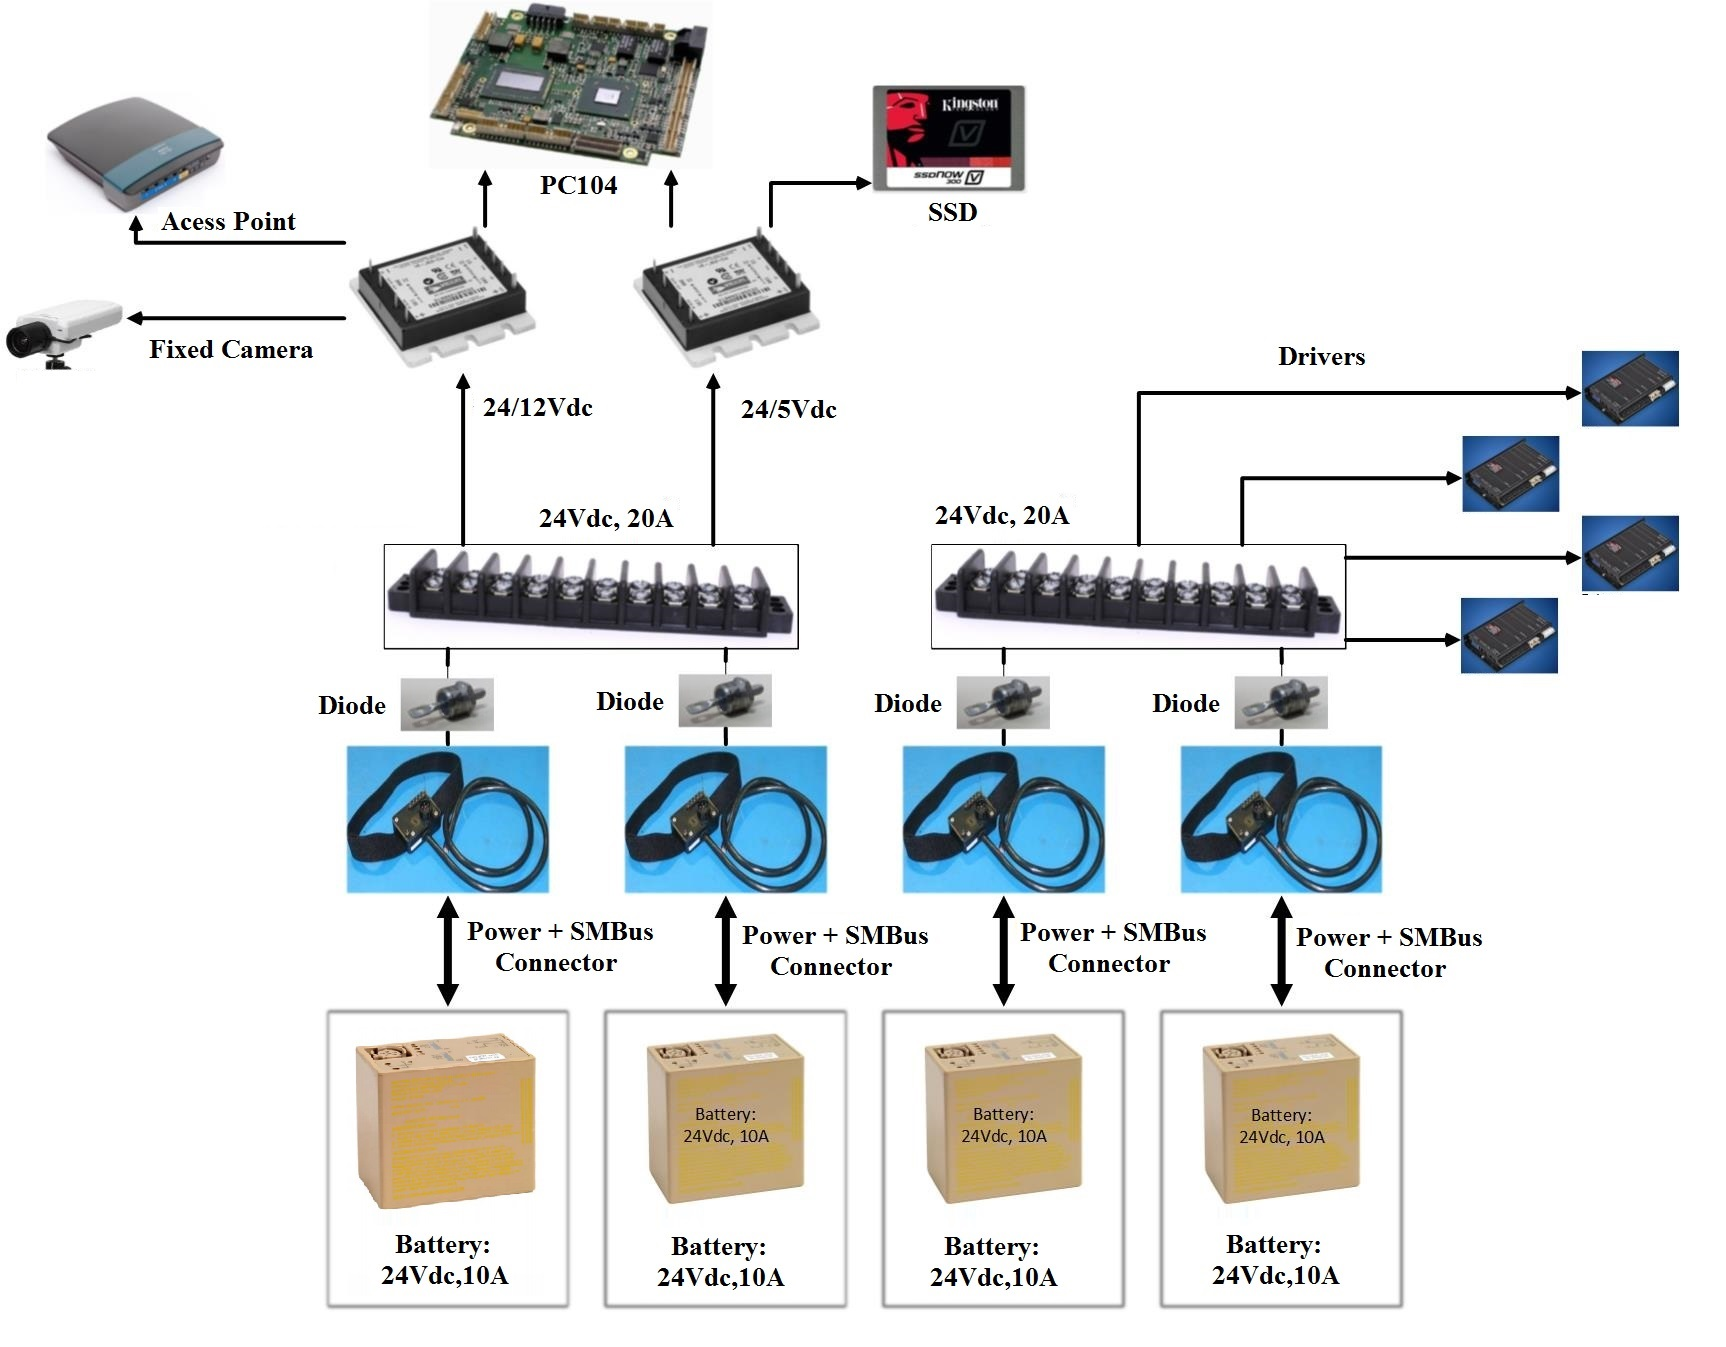
\includegraphics[width=1\columnwidth]{figs/DiagramaSAM.jpg}
\caption{DORIS power Supply Architecture.}
 \label{fig:DiagramaSAM}
\end{figure}

Considering this, new challenges arise in order to improve the features of
the system.

\section{Software System}\label{sec:software}

The software subsystem allows the implementation of high and low level control
of the robot. The DORIS software architecture considers two important factors:
all tools have to be open-source, and they have provide modular functionalities.
These requirements led to the adoption of Qt as the graphical interface
framework (\cite{qt}), Robot Operating System (ROS) as the communication
middleware (\cite{ros}), and Linux/Ubuntu as the operating system.


The software provides autonomous control (programmed tasks) and remote control
through a Graphical User Interface (GUI) in the Host Control Base (HCB)
computer. In both computers (Robot and HCB) a set of processes, denominated ROS
nodes, are running in parallel and they can communicate with each other through
ROS. To deal with this specification, a software framework, called Robot
Package Software is proposed, which is based on tools (graphical windows) and
components (processing and communication unities), and grouping them into a
dynamic library, libRobotPackage.so. The Robot Package is a general package
which can be re-used for another robotics systems. Additionally, a more specific
package, DORIS Package, is proposed to deal with Doris hardware and
functionalities. DORIS Package is a library (libDORISPackage.so) containing a
list of components and tools for the DORIS robot.

A robot system 3D model based on URDF format from ROS is
presented in figure~\ref{fig:rviz}.
The 3D model which include the rail and the robot system is integrated in the GUI and can be
visualized using RVIZ (a ROS tool).  Thus, the robot motion can be visualized
in the GUI and the operator can even control the robot in the 3D environment,
pointing a desided configuration.

\begin{figure}[!h]
\centering
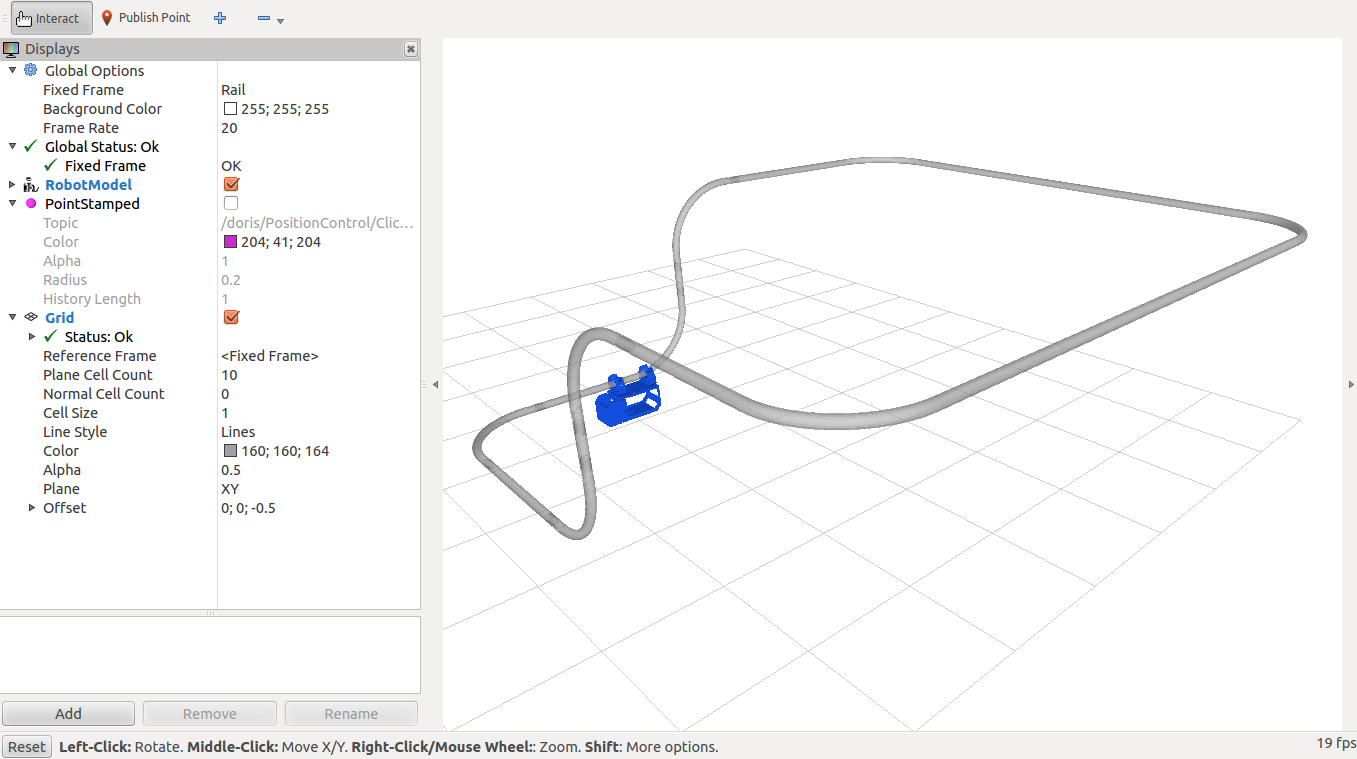
\includegraphics[width=8.4cm]{figs/rviz.png}
\caption{Robot system 3D model}
\label{fig:rviz}
\end{figure}

A Web tool is also proposed to remotly control DORIS using an standard internet
browser with javascript support (figure~\ref{fig:teleop}). The webtool is based
on rosbridge and javascript libraries roslibjs, ros2js and ros3djs.

\begin{figure}[!h]
\centering
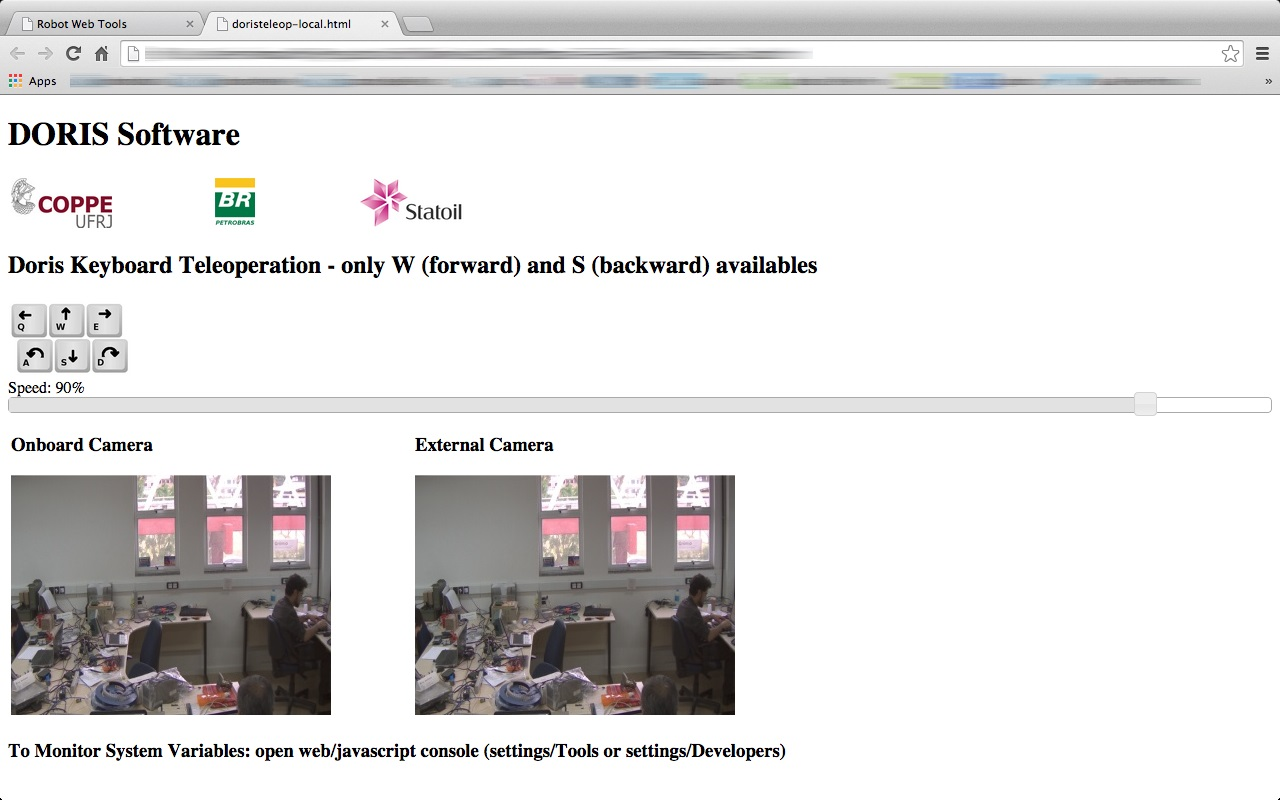
\includegraphics[width=8.4cm]{figs/teleop.jpg}
\caption{Web tool to remotly control DORIS using an standard internet
browser}
\label{fig:teleop}
\end{figure}


\section{Experimental tests and results}\label{sec:results}
A DORIS prototype named \emph{Single Autonomous Module} (SAM) was built for
tests of all concepts above. In addition, some VSS functionalities were
individually tested, but not yet fully integrated with SAM. The two subsections
below detail the tests.

\subsection{Single Autonomous Module (SAM)}
SAM (figure~\ref{fig:SAM2}) is a module composed mainly of AXIS ethernet fixed
camera, USB Minoru 3D Webcam, Cisco wireless router, four EC-4pole 200 W motors and
Maxon EPOS drivers, a PCIe/104 pentium i7 computer module with \emph{solid-state drive}
(Kingston SSD) and few PCBs. It was tested in horizontal and vertical motion on
a closed rail composed of straight and curved PVC tubes. The track comprises
all possible movements that the robot must make, and was installed in the
GSCAR laboratory, in COPPE/UFRJ. The robot was able to fully move throughout
the entire track.

The first objectives of SAM are to test the following concepts:
\begin{itemize}
  \item Power supply: independent buses for motors and electronics devices;
  batteries robustness and duration;
  \item Electronics: sensor integration; communication system;
  \item Software: teleoperation; user interface.
  \end{itemize}

\begin{figure}[!h]
\centering
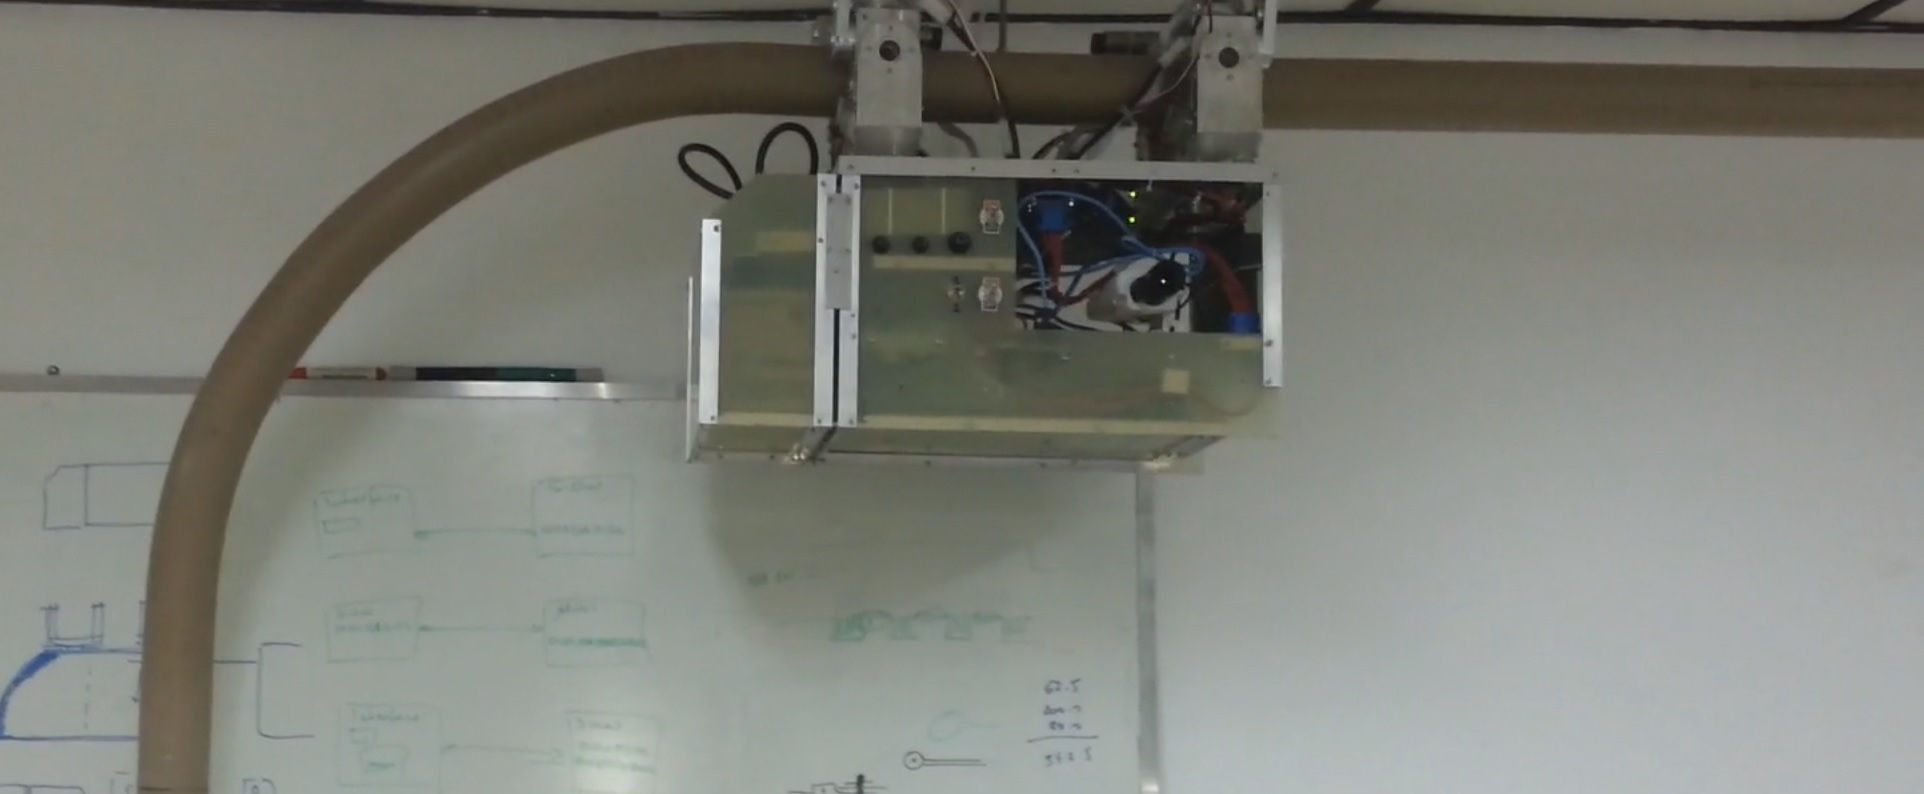
\includegraphics[width=8.4cm]{figs/SAM4.jpg}
\caption{Single Autonomous Module}
\label{fig:SAM2}
\end{figure}

The concept of independent power buses proved to be efficient, and the designed
battery capacity could handle the system energy demand. However, it was
observed that when SAM moves downwards, the motor rotates on the opposite
direction and through that energy is regenerated on the way back to the source.
Depending on the length of the downwards section and the robot velocity, this energy may reach a
voltage level that causes the motor drivers to reset, where this issue must
have further studies in order to investigate if it would be more worth to store
this extra energy or to simply waste it using an addicional device to burn it.

The implemented communication networks were: i) Ethernet, to connect the fixed
camera, the PCIe/104 and the access point; ii) Wi-Fi, to connect SAM with the
base; iii) CAN, to control the actuation system; iv) USB, to connect the 3D
Webcam. The communications worked
properly as expected.

It was proven that SAM can be teleoperated from anywhere by accessing its Wi-Fi
network and the GUI (\emph{Graphical User Interface}) developed in Qt
environment. SAM has already been teleoperated from CENPES/Petrobras (Rio de
Janeiro) and from Statoil headquarters (Norway).

\subsection{Vehicle Support System Tests}
All DORIS VSS functions were successfully tested independently. For these
tests, it was used a test PCB (similar to the designed for the final
prototype) and a RS485 interface with a notebook to emulate the USART
communication. The AVR firmware was programmed in C++ using Atmel Studio 6.1.
The following tests/implementations were successfully performed:
\begin{enumerate}[i)]
\item Logic for commanding the \emph{solid-state relays} for device on/off: the
relays can be opened/closed via RS485 commands from the laptop.
\item Acquisition of \emph{module voltages}: DC-DC voltage measurements (5, 12
and 24 VDC) and battery raw voltage measurement (that does not pass through any
DC-DC) can be accessed via RS485 commands from the laptop. The voltage is
measured using the AVR embedded AD converter.
\item Acquisition of \emph{module currents}: the measurement of currents that
supply each device module can be read via RS485 commands from the notebook. The
currents are measured using hall-effect sensors. The microcontroller embedded
AD converter does not comport enough measuring ports, thus an external one is
used to digitalize the current measurements.
\item Acquisition of \emph{module humidity/temperature}: the measurements of
the module humidity and temperature can be read via RS485 commands from the
notebook. A specific T/H sensor is used for this acquisition.
\item Acquisition of \emph{battery information}: voltages, temperature,
currents, remaining charge, and battery status, can be read via RS485 commands
from the notebook. The acquisition of all battery data is implemented using
SMBUS communication.   
\end{enumerate}

Future work include: replace RS485 by USART to allow communication with
the PCs via Ethernet network; implement in AVR the control of BMS high-power
relays to allow the management of DORIS energy power distribution; implement
the logic that uses the data read from SMBUS to manage DORIS energy
distribution. Additionally, timers will be implemented to enable: robot
shutdown in predetermined time; periodic data report of voltages,
currents, relays’ status, and module humidity and temperature.


\section{Conclusion and Future work}\label{sec:conclusions}

In this paper, we presented the embedded electronics subsystem of the DORIS
project, which endeavors to develop an offshore facilities inspection and monitoring robot. The prototype is based on
rail guided modules powered by a battery system and equipped with multiple
sensors that enable the detection of anomalies, such as abandoned objects and
gas leakage.

A prototype, SAM, was built to test electronics, power
supply, and software architecture concepts.
Preliminary results show good overall performance of: i) sensor integration and
communication; ii) independent power buses for electronics and motors; iii)
teleoperation.

The Vehicle Support System was tested outside the robot and the customized
printed circuit boards were able to monitor: the batteries via SMBUS,
temperature/humidity, DC/DC voltage levels, and devices's currents. The
solid-state relays can also turn on/off the devices for protection and/or
efficiently power consumption.

Ongoing implementations and future challenges include:
\begin{enumerate}[i)]
  \item \emph{Expansion and reconfiguration of robot modules}:\\
  \newline
  DORIS will need more than one module to support more devices and features.
  The EE system permits the free expansion and reconfiguration of DORIS
  modules, achieved by the use of a bus topology for DORIS
  main networks: Ethernet and CAN.\\
  \item \emph{Autonomous operation}:\\
  \newline
  DORIS autonomous operation is a challenge for the software development. The
  Positioning System, comprising wheels' encoders (odometry) and
  fixed camera (3D mapping), will be upgraded with an inertial movement unit
  (IMU) and the detection of rail landmarks, such as rail supports and segments connections. The fusion of these sensors measurements will estimate the vehicle states, such as position, attitude and velocity.
  %Melhorar isso ai
  %Also, a Mission Control System need to be developed for the operator.\\
\newline	
  \item \emph{Reduced interferences, such as electromagnetic interference (EMI)
  and electrostatic charge}:\\
  \newline
  Future DORIS improvements should include a well designed/installation of the
  shield network and grounding system to reduce EMI. An electrostatic discharger
  should be designed to drain the accumulated charge from the shielding system.\\
  \newline
  \item \emph{Solution for DORIS's downward motion issue}\\
  \newline
  The regeneration issue impose an overvoltage on the drivers, which resets for
  a while during the robot movement downwards. To prevent it, a shunt regulator
  may be used in order to dispose the extra energy and avoid the over
  voltage issue. It represents a solution, but wastes this energy, while a
  big capacitor bank could be used as an energy storage device. Tests are going
  to be performed so that the amount of energy generated may be measured in
  order to decide if it would be worth to embed a device to recover this
  energy or if it would be better just to let it be wasted.
  \newline
  \item \emph{Hardware Certification}\\
  \newline
  The robot must be certified to operate in corrosive environments and explosive
  atmospheres.
\end{enumerate}

\bibliography{ifacconf}

\appendix

\end{document}
